\documentclass[aspectratio=169]{beamer}
%% deck-source-version: 1
% ---- ツール管理プリアンブル(将来は deck init / deck format が生成・所有する)----
\usetheme{default}
\setbeamertemplate{navigation symbols}{}
\usepackage{graphicx}
\usepackage{amsmath}
\usepackage{amssymb}
\usepackage{booktabs}
\usepackage{hyperref}
% ---- ツール管理ここまで ----

%% macros:begin
%% macros:end

%% preamble-extra:begin
%% preamble-extra:end

\title{A Tiny Study of Deck Editing}
\subtitle{Golden sample: subset vocabulary only}
\author{Beamer Editor Team}
\institute{Slide Tools Lab}
\date{2026-07-10}

\begin{document}

\begin{frame}
  \titlepage
\end{frame}

\begin{frame}{Outline}
  \tableofcontents
\end{frame}

\section{Introduction}

\begin{frame}{Motivation}
  \begin{itemize}
    \item Slides should be a shared language between humans and AI.
    \item Binary formats hide structure.
      \begin{itemize}
        \item Diff review becomes impossible.
        \item Instructions get ambiguous.
          \begin{itemize}
            \item Three levels of nesting are allowed.
          \end{itemize}
      \end{itemize}
    \item Plain LaTeX lacks a live preview.
  \end{itemize}
\end{frame}

\begin{frame}{Steps with overlays}
  \begin{enumerate}
    \item<1-> Parse the source.
    \item<2-> Render the preview.
    \item<3> Ship the PDF.
    \item<2,4> This item shows on steps two and four.
  \end{enumerate}
\end{frame}

\begin{frame}{Pause demo}
  First we show this line.
  \pause
  Then this one appears.
\end{frame}

\section{Design}

\begin{frame}{Two columns}
  \begin{columns}[T]
    \begin{column}{0.5\textwidth}
      \begin{itemize}
        \item Left side takes half the width.
        \item Widths are factors of the text width.
      \end{itemize}
    \end{column}
    \begin{column}{0.45\textwidth}
      Right side is prose with \emph{emphasis} and a bit of $x^2$ math.
    \end{column}
  \end{columns}
\end{frame}

\begin{frame}{Blocks}
  \begin{block}{Definition}
    A deck is a single compilable file.
  \end{block}
  \begin{alertblock}{Warning}
    The HTML preview is an approximation; the PDF is the authority.
  \end{alertblock}
  \begin{exampleblock}<2->{Example}
    This example block appears on step two.
  \end{exampleblock}
\end{frame}

\begin{frame}{An image}
  \begin{center}
    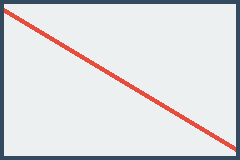
\includegraphics[width=0.4\textwidth]{assets/logo.png}
  \end{center}
\end{frame}

\begin{frame}{Results table}
  \begin{center}
    \begin{tabular}{lcr}
      \toprule
      Method & Accuracy & Time \\
      \midrule
      Baseline & 71.2 & 0.8 \\
      Ours & \textbf{79.6} & 1.1 \\
      \bottomrule
    \end{tabular}
  \end{center}
\end{frame}

\begin{frame}{Mathematics}
  Inline math like $e^{i\pi} + 1 = 0$ and \(\textstyle\sum_{k=1}^{n} k\) both work.
  \[
    f(x) = \int_{-\infty}^{x} e^{-t^{2}} \, dt
  \]
  \begin{equation*}
    \nabla \cdot \mathbf{E} = \frac{\rho}{\varepsilon_{0}}
  \end{equation*}
  \begin{align*}
    (a + b)^{2} &= a^{2} + 2ab + b^{2} \\
    (a - b)^{2} &= a^{2} - 2ab + b^{2}
  \end{align*}
\end{frame}

\begin{frame}{Inline vocabulary}
  We support \textbf{bold}, \emph{emphasis}, \textit{italics}, \texttt{monospace},
  and \alert{alerts}, plus \textcolor{blue}{named colors}.\\
  Links: \url{https://example.com} and \href{https://example.com}{a labelled link}.\\
  Special characters: 100\% done, R\&D, snake\_case, item \#1, \{braces\},
  a~non-breaking space, an en--dash, an em---dash.
\end{frame}

\section{Evaluation}

\subsection{Quantitative}

\begin{frame}[label=results]{Key results}
  % このフレームは label 付き(永続アドレスのサンプル)
  \begin{itemize}
    \item Accuracy improved by \textbf{8.4 points}.
    \item Latency stayed under one second.
  \end{itemize}
\end{frame}

\begin{frame}[allowframebreaks]{Related work}
  \begin{itemize}
    \item Presentation DSLs compile to slides but hide the output language.
    \item WYSIWYG editors lose the diffable source.
    \item Subset editors keep both, at the cost of a smaller vocabulary.
  \end{itemize}
\end{frame}

\begin{frame}[plain]
  \begin{center}
    A plain frame without decorations.
  \end{center}
\end{frame}

\begin{frame}{Summary}
  \begin{itemize}
    \item One source, three writers: human, AI, GUI.
    \item The subset is small enough to parse and large enough to present.
  \end{itemize}
\end{frame}

\end{document}
